\section{Evaluation}


The original goal of the project is to create a scalable logging algorithm that does not act as a bottleneck for the database as a whole. The data shown below was collected to determine the scalability of the algorithm. \par

The results in figure~\ref{serialresults} are used to show the scalability of the serial logging algorithm with and without the  opitimization described earlier.  The graph indicates the amount of time one txn would take to log. The goals are to minimize the amount the time increases as the thread count increases, indicating high scalability and decreasing the average log time per transaction. Each experiment  was tested on a maximum of 10000 txns and buffer sizes ranging from 10 to 100. 10 tests were run for each buffer size, and the average of these 10 test are shown below. \par 

\begin{figure}[!h]
  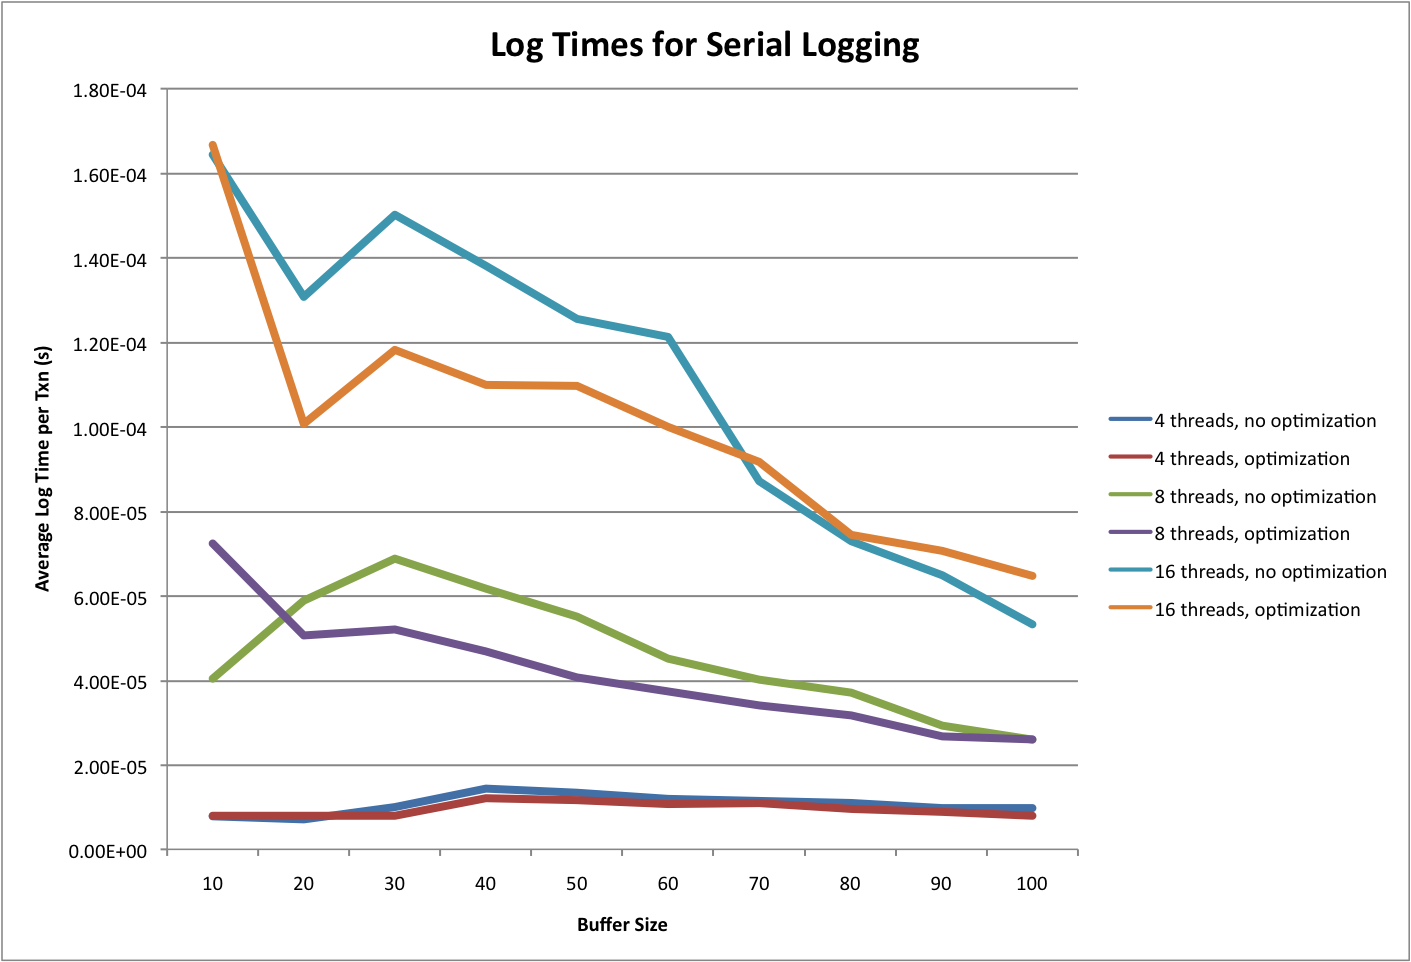
\includegraphics[width=\textwidth]{results.png}
  \caption{Serial logging results}
  \label{serialresults}
\end{figure}\\

The results from figure~\ref{serialresults} do not portray the deseired scalability. As thread size increases, the average log time per txn increases dramatically as well. As the thread count increases, however, the buffer size becomes more important, and a larger buffer size yields a lower average log time per transaction, which is desired. This trend is oberserved because a larger buffer size man that more data is being put on the buffer, limiting the number of times buffers must flush to the disk. The disk is slow, so the number of times the disk is access should be minimzied. As thread count increases, the number of times buffers must be flushed also increases, meaning that a larger buffer size becomes more important with an increase in thread count. \par

%BATCH LOGGING RESULTS
After testing the scalability of serial logging, batch logging was tested to determine its effieciency. Various implementations of batch logging were tesed with a different number of loggers. The average total run time and average time spent logging were recorded and graphed. Since we want to reduce run and logging times, lower is better. We expected an increase in the number of loggers to correspond with faster run and logging times, and the results back that hypothesis.
\begin{figure}
	\caption{Batch Logging Results}
	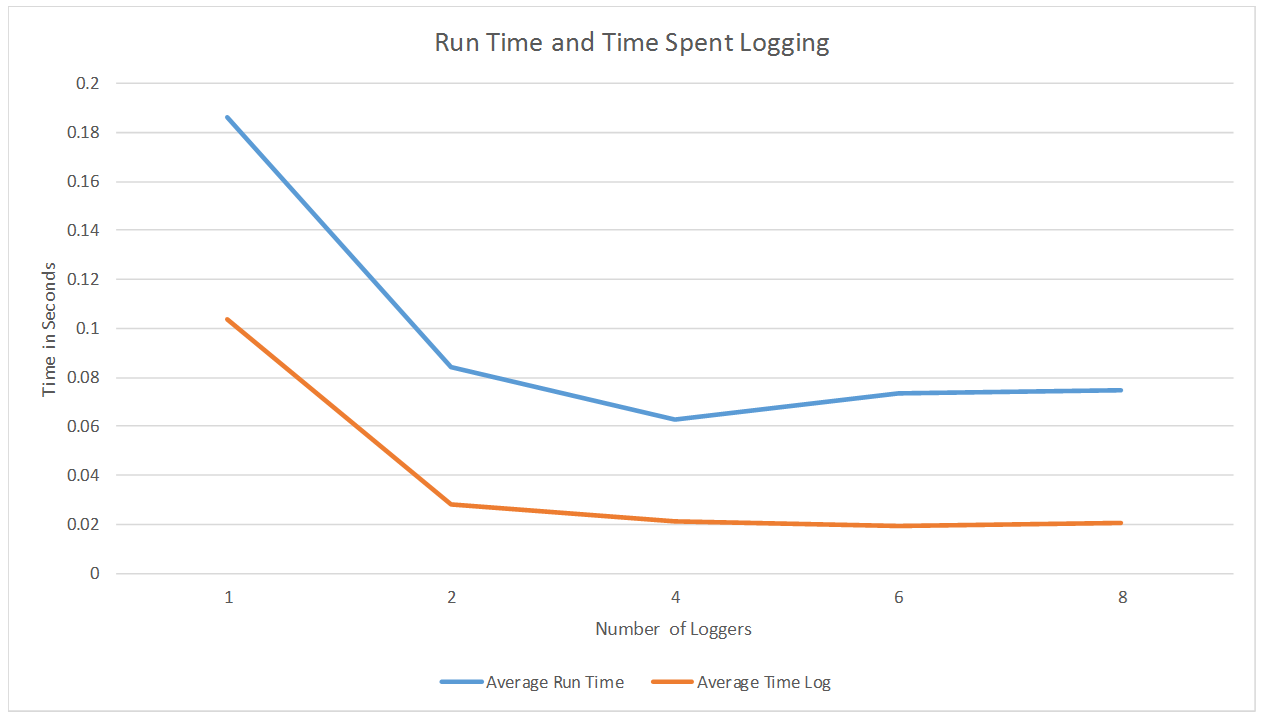
\includegraphics[width=\textwidth]{BatchLoggingResults.png}
\end{figure}
